
\section{Devices Information Model}
\label{sec:Devices Information Model}

The \gls{Devices Information Model} provides a representation of the physical and logical configuration for a piece of equipment used for a manufacturing process or for any other purpose.  It also provides the definition of data that may be reported by that equipment. 

Using information defined in the \gls{Devices Information Model}, a software application can determine the configuration and reporting capabilities of a piece of equipment.  To do this, the software application issues a \gls{Probe Request} (defined in \citetitle{MTCPart1} to an \gls{Agent} associated with a piece of equipment. An \gls{Agent} responds to the \gls{Probe Request} with an \gls{MTConnectDevices Response Document} that contains information describing both the physical and logical structure of the piece of equipment and a detailed description of each \gls{Data Entity} that can be reported by the \gls{Agent} associated with the piece of equipment. This information allows the client software application to interpret the document and to extract the data with the same meaning, value, and context that it had at its original source.  

The \gls{MTConnectDevices Response Document} is comprised of two sections: \block{Header} and \block{Devices}.

The \block{Header} section contains protocol related information as defined in \citetitle{MTCPart1} \textit{Section 6.5.1}.

The \block{Devices} section of the \gls{MTConnectDevices Response Document} contains a \block{Device} element for each piece of equipment described in the document.  Each \block{Device} is comprised of two primary types of elements - \glspl{Structural Element} and \glspl{Data Entity}.  

\glspl{Structural Element} organize information that represents the physical and logical parts and sub-parts of a piece of equipment (See \sect{Structural Elements for MTConnectDevices} for more details).  

\glspl{Data Entity} describe data that can be reported by a piece of equipment.  In the \gls{Devices Information Model}, \glspl{Data Entity} are defined as \block{DataItem} elements (See \sect{DataItem Types} and \sect{DataItem SubTypes}).

The \glspl{Structural Element} and \glspl{Data Entity} in the \gls{MTConnectDevices Response Document} provide information representing the physical and logical structure for a piece of equipment and the types of data that the piece of equipment can report relative to that structure.   The \gls{MTConnectDevices Response Document} does not contain values for the data types reported by the piece of equipment.  The \gls{MTConnectStreams Response Document} defined in \citetitle{MTCPart3} provides the data values that are reported by the piece of equipment.

\begin{note}
Note:  The \gls{MTConnect Standard} also defines the information model for \glspl{Asset}.  An \gls{Asset} is something that is used in the manufacturing process, but is not permanently associated with a single piece of equipment, can be removed from the piece of equipment without compromising its function, and can be associated with other pieces of equipment during its lifecycle.  See \citetitle{MTCPart40} for more details on \glspl{Asset}.

\end{note}

\section{Structural Elements for MTConnectDevices}
\label{sec:Structural Elements for MTConnectDevices}

\glspl{Structural Element} form the logical structure for the \gls{MTConnectDevices Response Document}.  These elements are used to organize information that represents the physical and logical architecture of a piece of equipment.  Refer to {{fig(MTConnectDevices Structural Elements}} for an overview of the \glspl{Structural Element} used in an \block{MTConnectDevices} document.

\begin{figure}[ht]
  \centering
    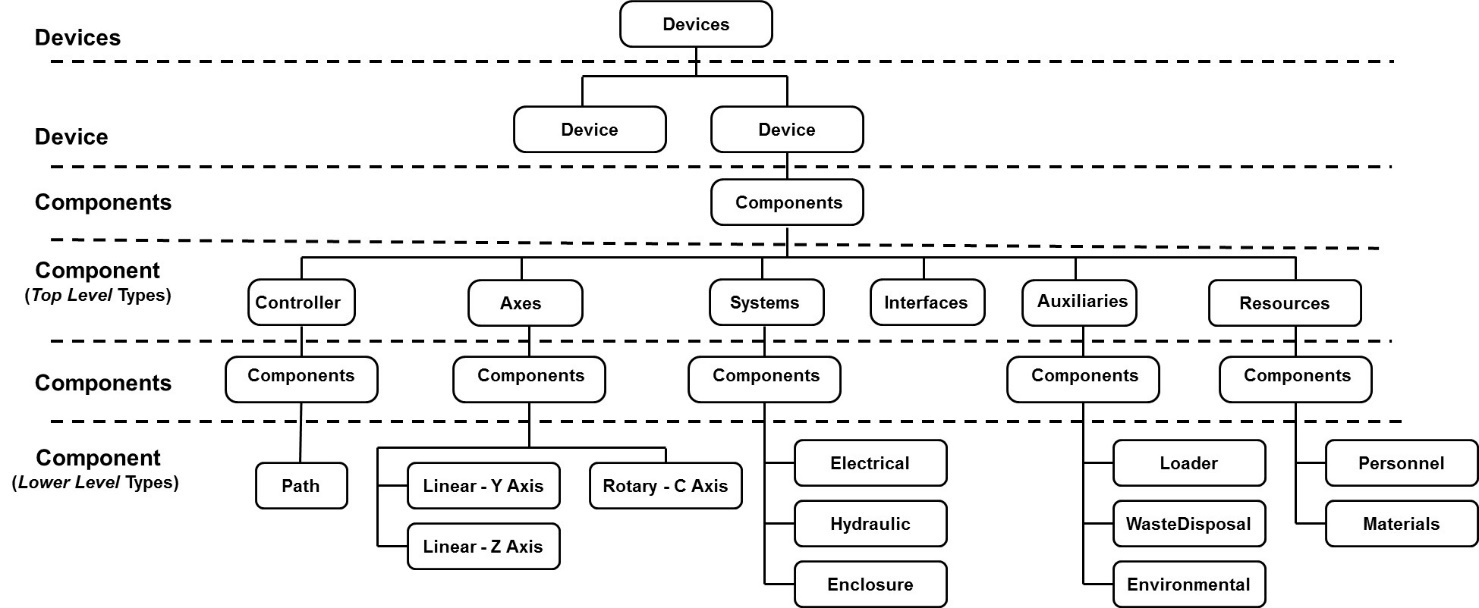
\includegraphics[width=1.0\textwidth]{figures/MTConnectDevices Structural Elements.png}
  \caption{MTConnectDevices Structural Elements Diagram}
  \label{fig:MTConnectDevices Structural Elements}
\end{figure}

\FloatBarrier


A variety of \glspl{Structural Element} are defined to describe a piece of equipment.  Some of these elements \textbf{MUST} always appear in the \block{MTConnectDevices} document, while others are optional and \textbf{MAY} be used, as required, to provide additional structure.

The first, or highest level, \gls{Structural Element} in a \block{MTConnectDevices} document is \block{Devices}. \block{Devices} is used to group one or more pieces of equipment into a single document.  \block{Devices} \textbf{MUST} always appear in the \block{MTConnectDevices} document.

\block{Device} is the next \gls{Structural Element} in the \block{MTConnectDevices} document. A separate \block{Device} element is used to identify each piece of equipment represented in the \block{MTConnectDevices} document. Each \block{Device} provides information on the physical and logical structure of the piece of equipment and the data associated with that equipment. \block{Device} can also represent any logical grouping of pieces of equipment that function as a unit or any other data source that provides data through a \gls{Agent}.

One or more \block{Device} element(s) \textbf{MUST} always appear in an \block{MTConnectDevices} document.

\block{Components} is the next \gls{Structural Element} in the \block{MTConnectDevices} document. \block{Components} is used to group information describing \gls{Lower Level} physical parts or logical functions of a piece of equipment.

If the \block{Components} in the document, it \textbf{MUST} contain one or more \block{Component} elements.

\block{Component} is the next level of \gls{Structural Element} in the \block{MTConnectDevices} document. \block{Component} is both an abstract type element and an \gls{organizer} type element. 

As an abstract type element, \block{Component} will never appear in the document describing a piece of equipment and will be replaced by a specific \block{Component} type defined in \sect{Component Types}. Each \block{Component} can also be used to organize information describing \gls{Lower Level} \glspl{Structural Element} or \glspl{Data Entity} associated with the \block{Component}.

If \gls{Lower Level} \glspl{Structural Element} are described, these elements are by definition child \block{Component} elements of a parent \block{Component}. At this next level, the \gls{Lower Level} child \block{Component} elements are grouped into an \gls{organizer} element called \block{Components}.
 
This \gls{Lower Level} \block{Components} container is comprised of one or more child \block{Component} elements representing the sub-parts of the parent \block{Component}. Just like the parent \block{Component} element, the child \block{Component} element is an abstract type element and will never appear in the document – only the different \gls{Lower Level} child \block{Component} types will appear.

This parent-child relationship can continue to any depth required to fully define a piece of equipment.

\input model-sections/Components.tex

\input model-sections/Devices.tex

\input model-sections/ComponentTypes.tex

\section{Compositions}
\label{sec:Compositions}

\block{Composition} \glspl{Structural Element} are used to describe the lowest level physical building blocks of a piece of equipment contained within a \block{Component}. By referencing a specific \block{Composition} element, further clarification and meaning to data associated with a specific \block{Component} can be achieved.

Both \block{Component} and \block{Composition} elements are \gls{Lower Level} child \block{Component} \gls{XML} elements representing the sub-parts of the parent \block{Component}.  However, there are distinct differences between \block{Component} and \block{Composition} type elements.

\block{Component} elements may be further defined with \gls{Lower Level} \block{Component} elements and may have associated \glspl{Data Entity}.

\block{Composition} elements represent the lowest level physical part of a piece of equipment.  They \textbf{MUST NOT} be further defined with \gls{Lower Level} \block{Component} elements and they \textbf{MUST NOT} have \glspl{Data Entity} directly associated with them.   They do provide additional information that can be used to enhance the specificity of \glspl{Data Entity} associated with the parent \block{Component}.

\input model-sections/Compositions.tex

\input model-sections/CompositionTypes.tex

\section{DataItems}
\label{sec:DataItems}

In the \block{MTConnectDevices} document, \glspl{Data Entity} describe data that can be reported by a piece of equipment and are associated with \block{Device} and \block{Component} \glspl{Structural Element}.   While the \glspl{Data Entity} describe the data that can be reported by a piece of equipment in the \block{MTConnectDevices} document, the actual data values are provided in the \gls{Streams Information Model}.   See \citetitle{MTCPart3} for detail on the reported values.

Each \gls{Data Entity} \textbf{SHOULD} be modeled in the \block{MTConnectDevices} document such that it is associated with the \gls{Structural Element} that the reported data directly applies.

When \glspl{Data Entity} are associated with a \gls{Structural Element}, they are organized in a \block{DataItems} element.   \block{DataItems} provides the structure for organizing individual \block{DataItem} elements that represent each \gls{Data Entity}. \block{DataItems} is comprised of one or more \block{DataItem} type element(s).

\block{DataItem} describes specific types of \glspl{Data Entity} that represent a numeric value, a functioning state, or a health status reported by a piece of equipment. \block{DataItem} provides a detailed description for each \gls{Data Entity} that is reported; it defines the type of data being reported and an array of optional attributes that further describe that data.   The different types of \block{DataItem} elements are defined in \sect{DataItem Types}.

\input model-sections/DataItems.tex

\input model-sections/ElementsforDataItem.tex

\input model-sections/ElementsforDefinition.tex

\input model-sections/DataItemTypes.tex

\input model-sections/DataItemSubTypes.tex

\section{References}
\label{sec:References}

\block{References} organizes pointers to information defined elsewhere for a piece of equipment.

\block{References} may be modeled as part of a \block{Device}, \block{Component} or \block{Interface} type \gls{Structural Element}.

\input model-sections/References.tex

\section{Configuration}
\label{sec:Configuration}

This section provides semantic information for \block{Configuration} and its types.

\begin{figure}[ht]
  \centering
    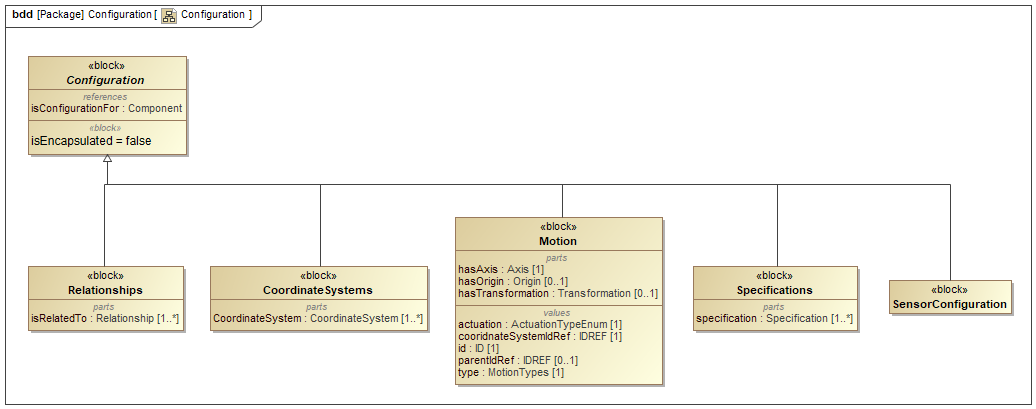
\includegraphics[width=1.0\textwidth]{figures/Configuration.png}
  \caption{Configuration Diagram}
  \label{fig:Configuration}
\end{figure}

\FloatBarrier

\input model-sections/Configuration.tex

\input model-sections/CoordinateSystems.tex

\input model-sections/Motion.tex

\input model-sections/Relationships.tex

\input model-sections/Sensor.tex

\input model-sections/Specifications.tex
